% Options for packages loaded elsewhere
\PassOptionsToPackage{unicode}{hyperref}
\PassOptionsToPackage{hyphens}{url}
%
\documentclass[
]{report}
\usepackage{amsmath,amssymb}
\usepackage{lmodern}
\usepackage{iftex}
\ifPDFTeX
  \usepackage[T1]{fontenc}
  \usepackage[utf8]{inputenc}
  \usepackage{textcomp} % provide euro and other symbols
\else % if luatex or xetex
  \usepackage{unicode-math}
  \defaultfontfeatures{Scale=MatchLowercase}
  \defaultfontfeatures[\rmfamily]{Ligatures=TeX,Scale=1}
\fi
% Use upquote if available, for straight quotes in verbatim environments
\IfFileExists{upquote.sty}{\usepackage{upquote}}{}
\IfFileExists{microtype.sty}{% use microtype if available
  \usepackage[]{microtype}
  \UseMicrotypeSet[protrusion]{basicmath} % disable protrusion for tt fonts
}{}
\makeatletter
\@ifundefined{KOMAClassName}{% if non-KOMA class
  \IfFileExists{parskip.sty}{%
    \usepackage{parskip}
  }{% else
    \setlength{\parindent}{0pt}
    \setlength{\parskip}{6pt plus 2pt minus 1pt}}
}{% if KOMA class
  \KOMAoptions{parskip=half}}
\makeatother
\usepackage{xcolor}
\usepackage{color}
\usepackage{fancyvrb}
\newcommand{\VerbBar}{|}
\newcommand{\VERB}{\Verb[commandchars=\\\{\}]}
\DefineVerbatimEnvironment{Highlighting}{Verbatim}{commandchars=\\\{\}}
% Add ',fontsize=\small' for more characters per line
\usepackage{framed}
\definecolor{shadecolor}{RGB}{248,248,248}
\newenvironment{Shaded}{\begin{snugshade}}{\end{snugshade}}
\newcommand{\AlertTok}[1]{\textcolor[rgb]{0.94,0.16,0.16}{#1}}
\newcommand{\AnnotationTok}[1]{\textcolor[rgb]{0.56,0.35,0.01}{\textbf{\textit{#1}}}}
\newcommand{\AttributeTok}[1]{\textcolor[rgb]{0.77,0.63,0.00}{#1}}
\newcommand{\BaseNTok}[1]{\textcolor[rgb]{0.00,0.00,0.81}{#1}}
\newcommand{\BuiltInTok}[1]{#1}
\newcommand{\CharTok}[1]{\textcolor[rgb]{0.31,0.60,0.02}{#1}}
\newcommand{\CommentTok}[1]{\textcolor[rgb]{0.56,0.35,0.01}{\textit{#1}}}
\newcommand{\CommentVarTok}[1]{\textcolor[rgb]{0.56,0.35,0.01}{\textbf{\textit{#1}}}}
\newcommand{\ConstantTok}[1]{\textcolor[rgb]{0.00,0.00,0.00}{#1}}
\newcommand{\ControlFlowTok}[1]{\textcolor[rgb]{0.13,0.29,0.53}{\textbf{#1}}}
\newcommand{\DataTypeTok}[1]{\textcolor[rgb]{0.13,0.29,0.53}{#1}}
\newcommand{\DecValTok}[1]{\textcolor[rgb]{0.00,0.00,0.81}{#1}}
\newcommand{\DocumentationTok}[1]{\textcolor[rgb]{0.56,0.35,0.01}{\textbf{\textit{#1}}}}
\newcommand{\ErrorTok}[1]{\textcolor[rgb]{0.64,0.00,0.00}{\textbf{#1}}}
\newcommand{\ExtensionTok}[1]{#1}
\newcommand{\FloatTok}[1]{\textcolor[rgb]{0.00,0.00,0.81}{#1}}
\newcommand{\FunctionTok}[1]{\textcolor[rgb]{0.00,0.00,0.00}{#1}}
\newcommand{\ImportTok}[1]{#1}
\newcommand{\InformationTok}[1]{\textcolor[rgb]{0.56,0.35,0.01}{\textbf{\textit{#1}}}}
\newcommand{\KeywordTok}[1]{\textcolor[rgb]{0.13,0.29,0.53}{\textbf{#1}}}
\newcommand{\NormalTok}[1]{#1}
\newcommand{\OperatorTok}[1]{\textcolor[rgb]{0.81,0.36,0.00}{\textbf{#1}}}
\newcommand{\OtherTok}[1]{\textcolor[rgb]{0.56,0.35,0.01}{#1}}
\newcommand{\PreprocessorTok}[1]{\textcolor[rgb]{0.56,0.35,0.01}{\textit{#1}}}
\newcommand{\RegionMarkerTok}[1]{#1}
\newcommand{\SpecialCharTok}[1]{\textcolor[rgb]{0.00,0.00,0.00}{#1}}
\newcommand{\SpecialStringTok}[1]{\textcolor[rgb]{0.31,0.60,0.02}{#1}}
\newcommand{\StringTok}[1]{\textcolor[rgb]{0.31,0.60,0.02}{#1}}
\newcommand{\VariableTok}[1]{\textcolor[rgb]{0.00,0.00,0.00}{#1}}
\newcommand{\VerbatimStringTok}[1]{\textcolor[rgb]{0.31,0.60,0.02}{#1}}
\newcommand{\WarningTok}[1]{\textcolor[rgb]{0.56,0.35,0.01}{\textbf{\textit{#1}}}}
\usepackage{longtable,booktabs,array}
\usepackage{calc} % for calculating minipage widths
% Correct order of tables after \paragraph or \subparagraph
\usepackage{etoolbox}
\makeatletter
\patchcmd\longtable{\par}{\if@noskipsec\mbox{}\fi\par}{}{}
\makeatother
% Allow footnotes in longtable head/foot
\IfFileExists{footnotehyper.sty}{\usepackage{footnotehyper}}{\usepackage{footnote}}
\makesavenoteenv{longtable}
\usepackage{graphicx}
\makeatletter
\def\maxwidth{\ifdim\Gin@nat@width>\linewidth\linewidth\else\Gin@nat@width\fi}
\def\maxheight{\ifdim\Gin@nat@height>\textheight\textheight\else\Gin@nat@height\fi}
\makeatother
% Scale images if necessary, so that they will not overflow the page
% margins by default, and it is still possible to overwrite the defaults
% using explicit options in \includegraphics[width, height, ...]{}
\setkeys{Gin}{width=\maxwidth,height=\maxheight,keepaspectratio}
% Set default figure placement to htbp
\makeatletter
\def\fps@figure{htbp}
\makeatother
\setlength{\emergencystretch}{3em} % prevent overfull lines
\providecommand{\tightlist}{%
  \setlength{\itemsep}{0pt}\setlength{\parskip}{0pt}}
\setcounter{secnumdepth}{5}
\usepackage[utf8]{inputenc}
\usepackage[slovene]{babel}
\usepackage{booktabs}
\ifLuaTeX
  \usepackage{selnolig}  % disable illegal ligatures
\fi
\usepackage[]{natbib}
\bibliographystyle{plainnat}
\IfFileExists{bookmark.sty}{\usepackage{bookmark}}{\usepackage{hyperref}}
\IfFileExists{xurl.sty}{\usepackage{xurl}}{} % add URL line breaks if available
\urlstyle{same} % disable monospaced font for URLs
\hypersetup{
  pdftitle={Računalniški praktikum (fizika) - vaje},
  pdfauthor={Rok Kuk - kontakt@rokuk.org},
  hidelinks,
  pdfcreator={LaTeX via pandoc}}

\title{Računalniški praktikum (fizika) - vaje}
\author{Rok Kuk - \href{mailto:kontakt@rokuk.org}{\nolinkurl{kontakt@rokuk.org}}}
\date{2022-12-01}

\begin{document}
\maketitle

{
\setcounter{tocdepth}{1}
\tableofcontents
}
\hypertarget{o-strani}{%
\chapter*{O strani}\label{o-strani}}
\addcontentsline{toc}{chapter}{O strani}

Na tej strani so zbrani zapiski za vaje predmeta računalniški praktikum v 1. letniku študija fizike na Fakulteti za matematiko in fiziko Univerze v Ljubljani.

Zapiski so mišljeni le kot opora pri izvajanju vaj in ne obsegajo čisto vseh obravnavanih vsebin. Zapiski zato ne morejo nadomestiti obiskovanja predavanj in vaj.

\begin{center}\rule{0.5\linewidth}{0.5pt}\end{center}

Vsebina teh strani je objavljena pod licenco CC BY-NC-SA 4.0.
Markdown koda za strani je dostopna na \url{https://github.com/rokuk/rp-fiz-notes}

\hypertarget{namestitev-okolja-za-vaje}{%
\chapter{Namestitev okolja za vaje}\label{namestitev-okolja-za-vaje}}

Da na računalniku uporabljate Python in rešujete naloge je potrebno namestiti
nekaj programov. Spodaj je opisan okvirni postopek in pogoste težave pri nameščanju
programov. Če imate težave, je opis problema dobro pogooglati, sicer pa lahko seveda vprašate sošolce, pišite
asistentu ali postavite vprašanje na forumu.

\hypertarget{namestitev-pythona}{%
\section{Namestitev Pythona}\label{namestitev-pythona}}

\begin{enumerate}
\def\labelenumi{\arabic{enumi}.}
\tightlist
\item
  Namestite Python (najbolje kar verzijo 3.10) s te strani (zavihek \texttt{Downloads}): \url{https://www.python.org}. Ko poženete program za namestitev, v oknu, ki se odpre, odkljukajte ``Add Python 3.x to PATH''. Nato nadaljujte z namestitvijo (opcija ``Install now'').
\end{enumerate}

\begin{quote}
Če uporabljate Windows 7 ali še starejši Windows, boste morali namestiti
starejšo verzijo Pythona (npr. 3.8.9 ali manj). Najdete jo tule:
\url{https://www.python.org/downloads/}
\end{quote}

\begin{enumerate}
\def\labelenumi{\arabic{enumi}.}
\setcounter{enumi}{1}
\tightlist
\item
  Preverite ali se je Python uspešno namestil. Odprite program Ukazni poziv (Windows)
  ali Terminal (macOS/Linux), ki je že na vašem računalniku. V okno, ki se odpre
  vpišite ukaz \texttt{python\ -\/-version} in pritisnite tipko Enter. Če je Python
  uspešno nameščen, bi se vam v novi vrstici moralo izpisati \texttt{Python\ 3.x.y}
  (kjer je \texttt{x.y} verzija nameščenega Pythona).
\end{enumerate}

\begin{quote}
Če ste na Windowsu in ukaz \texttt{python\ -\/-version} ne izpiše verzije, ampak se vam izpiše napaka ali ``Python not found'', poskusite ukaz \texttt{py\ -\/-version}.
\end{quote}

\hypertarget{namestitev-visual-studio-code}{%
\section{Namestitev Visual Studio Code}\label{namestitev-visual-studio-code}}

\begin{enumerate}
\def\labelenumi{\arabic{enumi}.}
\setcounter{enumi}{2}
\tightlist
\item
  Namestite Visual Studio Code: \url{https://code.visualstudio.com}
\item
  Namestite Python extension. Odprite Visual Studio Code. Morda se vam bo v oknu VSCode pojavil zavihek z naslovom \texttt{Get\ Started}, ki ga lahko kar zaprete.
  Na levem robu okna kliknite na Extensions (ikona s štirimi kvadratki), vpišite \texttt{Python},
  izberite \texttt{Python} in na desni kliknite \texttt{Install}. Morda se bo odprlo okno
  \texttt{Get\ Started}, ki ga lahko zaprete.
\item
  Dobro je, da si nekje na računalniku ustvarite mapo, v katero boste shranjevali
  vso vašo kodo. V VSCode v meniju File kliknite \texttt{Open\ Folder...} in izberite to mapo.
  Morda se bo pojavilo okno, ki vas sprašuje, če zaupate avtorju datotek
  v tej mapi: kliknite Yes, ker sebi zaupate. Ustvarite novo datoteko
  (meni File \textgreater{} New File), jo shranite (meni File \textgreater{} Save) in jo poimenujte
  \texttt{test.py} (na Windowsu izberete \texttt{Save\ as\ type:\ Python}). Vsebina datoteke se vam
  odpre kot zavihek v VSCode. Vanj vpišite \texttt{print("Pozdravljen\ svet!")}. V desnem
  zgornjem kotu bi morali imeti gumb v obliki puščice, s katerim lahko poženete napisani program.
  Če ga nimate, si lahko namestite extension z imenom \texttt{Code\ Runner}. Sicer lahko
  program poženete tudi tako, da desno kliknete kjerkoli v območju urejevalnika besedila in nato v
  meniju, ki se pojavi, izberete \texttt{Run\ Python\ File\ in\ Terminal}. Ko poženete program,
  bi se vam v oknu terminala moralo izpisati ``Pozdravljen svet!''.
\item
  Priporočam, da vklopite tudi ``linter''. To je program, ki je del VSCode in
  v vaši kodi sproti preverja ali ste se kje zmotili. Ne ujame vseh možnih napak,
  mnoge zatipke pa zazna in vas nanje opozori, še preden poženete program, tako da jih podčrta.
  VSCode pritisnite Ctrl+Shift+P in vpišite ``linter'' (brez navednic), kliknite na
  \texttt{Python:\ Select\ Linter}. Pojavi se meni z več možnostmi za linter.
  Priporočam \texttt{flake8}, ki nas poleg napak opozori tudi na kršitve priporočil za stil
  PEP8. Izberete ga s tipko Enter. VSCode vas bo desno spodaj obvestil, da ta linter ni nameščen;
  namestite ga tako, da kliknete \texttt{Install} v tem obvestilu. Po nekaj sekundah bi se moral namestiti. Lahko ga preizkusite tako, da v datoteko s končnico .py nekaj narobe napišete npr. \texttt{prnt("Pozdravljen\ svet!")}
\end{enumerate}

VSCode ima veliko funkcionalnosti, ki nam lahko pomagajo pri programiranju.
Več o tem piše v uradni dokumentaciji: \url{https://code.visualstudio.com/docs/editor/codebasics}

\hypertarget{namestitev-paketa-numpy}{%
\section{Namestitev paketa Numpy}\label{namestitev-paketa-numpy}}

Potrebovali bomo še Pythonov paket Numpy. To je neke vrste dodatek za Python, ki nam omogoča lažje delo z vektorji in tabelami. Več o tem na prihodnjih vajah. Dodatne module za Python lahko nameščamo in odstranjujemo z modulom \texttt{pip}. To je modul, ki bi se moral avtomatsko namestiti skupaj s Pythonom.

\begin{enumerate}
\def\labelenumi{\arabic{enumi}.}
\setcounter{enumi}{6}
\tightlist
\item
  Najprej v Ukazni poziv / Terminal vpišite in izvršite ukaz \texttt{python\ -m\ pip\ -\/-version}
  (če ste na Windowsu boste morda dobili napako v stilu ``python ne obstaja'',
  v tem primeru poskusite izvršiti ukaz \texttt{py\ -m\ pip\ -\/-version}).
  Izpisati bi se vam moralo nekaj podobnega \texttt{pip\ X.Y.Z\ from\ ...\ (python\ 3.N.N)}.
\end{enumerate}

\begin{quote}
Več o tem na \url{https://pip.pypa.io/en/stable/getting-started/}
\end{quote}

Če se vam izpiše to, lahko nadaljujete na 8. korak, sicer berite naprej.
Če se vam izpiše nekaj v stilu ``pip ne obstaja'' ali ``command not found'',
morate namestiti Pythonov modul \texttt{pip}. To naredite z ukazom
\texttt{python\ -m\ ensurepip\ -\/-upgrade} (oz. na Windowsu morda \texttt{py\ -m\ ensurepip\ -\/-upgrade}).

\begin{quote}
Več informacij o nameščanju modula \texttt{pip} je na \url{https://pip.pypa.io/en/stable/installation/\#python}
\end{quote}

\begin{enumerate}
\def\labelenumi{\arabic{enumi}.}
\setcounter{enumi}{7}
\tightlist
\item
  Namestite Pythonov modul numpy. To naredite z ukazom \texttt{python\ -m\ pip\ install\ numpy}
  (oz. na Windowsu bo morda treba uporabiti \texttt{py\ -m\ pip\ install\ numpy}).
\end{enumerate}

\hypertarget{pogoste-teux17eave}{%
\section{Pogoste težave}\label{pogoste-teux17eave}}

\begin{itemize}
\item
  Če pri poganjanju programa dobite napako \texttt{no\ module\ named\ numpy}, to pomeni, da Numpy ni nameščen. Če ste ga že namestili, je morda težava, da ste ga namestili za napačno verzijo Pythona (glej spodnjo alinejo). Če ga še niste namestili, poskusite zgoraj opisani postopek.
\item
  Če imate na računalniku nameščenih več verzij Pythona (to so npr. mnogi računalniki z macOS) se lahko ``python'' v ukazni vrstici / terminalu nanaša na drugo verzijo, kot je tista, ki jo uporabljate za poganjanje svojih programov v VSCode. Katera verzija se uporablja v VSCode lahko izberete tako, da odprete katerokoli datoteko s končnico .py in kliknete na ``Python 3.x.y'' na spodnjem robu okna. Pokaže se okno z vsemi nameščenimi verzijami. Da namestite Numpy za določeno verzijo Pythona lahko poskusite ukaz \texttt{python3.10\ -m\ pip\ install\ numpy}, kjer 3.10 zamenjate z želeno verzijo Pythona. Na Windowsu bi moral delovati ukaz \texttt{py\ -3.10\ -m\ pip\ install\ numpy}.
\end{itemize}

\hypertarget{uvod-v-ptyhon}{%
\chapter{Uvod v Ptyhon}\label{uvod-v-ptyhon}}

Gradiva za to poglavje so:

\begin{itemize}
\tightlist
\item
  \url{https://automatetheboringstuff.com/2e/chapter1/}
\item
  \url{https://automatetheboringstuff.com/2e/chapter2/} (do poglavja \texttt{while\ loop\ statements})
\item
  \url{https://automatetheboringstuff.com/2e/chapter3/}
\item
  poglavje \texttt{Osnovni\ koncepti\ programiranja} v \url{https://lusy.fri.uni-lj.si/ucbenik/book/1201/index.html}
\item
  poglavje \texttt{Izdelava\ samostojnih\ programov\ in\ pogojni\ stavki} v \url{https://lusy.fri.uni-lj.si/ucbenik/book/1202/index.html}
\item
  poglavje \texttt{Funkcije}v \url{https://lusy.fri.uni-lj.si/ucbenik/book/1205/index.html}
\end{itemize}

\hypertarget{ux161tevila}.
Za vrstni red računanja operacij (če jih kombiniramo) veljajo enaka pravila kot
v matematiki.

\begin{Shaded}
\begin{Highlighting}[]
\NormalTok{celidel }\OperatorTok{=} \DecValTok{20} \OperatorTok{//} \DecValTok{8}
\NormalTok{ostanek }\OperatorTok{=} \DecValTok{20} \OperatorTok{\%} \DecValTok{8}
\BuiltInTok{print}\NormalTok{(celidel, ostanek)}
\end{Highlighting}
\end{Shaded}

\begin{verbatim}
## 2 4
\end{verbatim}

Za zaokroževanje števila \texttt{stevilo} uporabimo funkcijo \texttt{round(stevilo,\ d)}, ki število zaokroži na \texttt{d} decimalnih mest.

\hypertarget{logiux10dne-operacije}{%
\section{Logične operacije}\label{logiux10dne-operacije}}

Logične operacije s ključnimi besedami \texttt{and}, \texttt{or} in \texttt{not} ustrezajo operacijam v matematiki.

\begin{itemize}
\tightlist
\item
  \texttt{a\ and\ b} je True, če sta \texttt{a} in \texttt{b} enaka True, sicer je False
\item
  \texttt{a\ or\ b} je False, le če sta \texttt{a} in \texttt{b} enaka False
\item
  \texttt{not\ a} je True, če je \texttt{a} enak False, sicer je True
\end{itemize}

Logične operacije lahko kombiniramo. Vrstni red operacij lahko določimo z oklepaji.
Sicer ima operator \texttt{and} prednost pred \texttt{or}, \texttt{not} pa ima prednost pred obema.

\begin{Shaded}
\begin{Highlighting}[]
\NormalTok{a }\OperatorTok{=} \VariableTok{True}
\NormalTok{b }\OperatorTok{=} \VariableTok{True}
\NormalTok{c }\OperatorTok{=} \VariableTok{False}
\BuiltInTok{print}\NormalTok{((a }\KeywordTok{or}\NormalTok{ b) }\KeywordTok{and}\NormalTok{ (a }\KeywordTok{or}\NormalTok{ c))}
\end{Highlighting}
\end{Shaded}

\begin{verbatim}
## True
\end{verbatim}

V logičnih operacijah se število 0 obnaša kot False, ostala števila pa kot True.

\hypertarget{relacijski-operatorji}{%
\section{Relacijski operatorji}\label{relacijski-operatorji}}

Če relacija velja ima izraz vrednost True, sicer pa False.

\begin{itemize}
\tightlist
\item
  primerjava števil \texttt{a\ \textless{}\ b} ali \texttt{a\ \textless{}=\ b}
\item
  preverjanje enakosti \texttt{a\ ==\ b}
\item
  preverjanje različnosti (nista enaka) \texttt{a\ !=\ b}
\end{itemize}

Logične operacije in relacije so binarne. Binarna operacija se izvede med tem,
kar je na levi, in tem, kar je na desni.

\hypertarget{nekoliko-kompleksnejux161i-primer}{%
\section{Nekoliko kompleksnejši primer}\label{nekoliko-kompleksnejux161i-primer}}

Če želimo preveriti ali je spremenljivka \texttt{mesec} enaka 6 ali 7, ni prav, če napišemo

\begin{Shaded}
\begin{Highlighting}[]
\NormalTok{mesec }\OperatorTok{=} \DecValTok{4}
\NormalTok{rezultat }\OperatorTok{=}\NormalTok{ mesec }\OperatorTok{==} \DecValTok{6} \KeywordTok{or} \DecValTok{7}
\BuiltInTok{print}\NormalTok{(rezultat)}
\end{Highlighting}
\end{Shaded}

\begin{verbatim}
## 7
\end{verbatim}

V zgornjem izrazu se najprej izvede primerjava med \texttt{mesec} in 6. Ker 4 ni enako 6,
nam to da False. Nato se izvede operacija \texttt{or} med False in 7. Ker se 7 obnaša
kot True bi pričakovali, da dobimo True. Operacija \texttt{or} deluje tako, da vrne prvo
vrednost, ki ni False. Ponavadi primerjamo True in False vrednosti, zato ima
operacija rezultat True, če je ena od vrednosti True.
Na levi strani je pri nas False, na desni pa 7, zato ima celoten izraz desno
od enačaja vrednost 7 (ker je prva vrednost, ki ni False).

Pravilna rešitev bi bila

\begin{Shaded}
\begin{Highlighting}[]
\NormalTok{mesec }\OperatorTok{=} \DecValTok{4}
\NormalTok{rezultat }\OperatorTok{=}\NormalTok{ (mesec }\OperatorTok{==} \DecValTok{6}\NormalTok{) }\KeywordTok{or}\NormalTok{ (mesec }\OperatorTok{==} \DecValTok{7}\NormalTok{)}
\BuiltInTok{print}\NormalTok{(rezultat)}
\end{Highlighting}
\end{Shaded}

\begin{verbatim}
## False
\end{verbatim}

\hypertarget{zanke}{%
\chapter{Zanke}\label{zanke}}

Gradivi za to poglavje sta

\begin{itemize}
\tightlist
\item
  \url{https://automatetheboringstuff.com/2e/chapter2/} (poglavji \texttt{while\ loop\ statements} in \texttt{for\ loops})
\item
  poglavje \texttt{Zanke} v \url{https://lusy.fri.uni-lj.si/ucbenik/book/1203/index.html}
\end{itemize}

\hypertarget{zanka-for}{%
\section{Zanka for}\label{zanka-for}}

Zanko for uporabimo, ko vemo kolikokrat želimo nekaj ponoviti.

\begin{Shaded}
\begin{Highlighting}[]
\NormalTok{zacetek }\OperatorTok{=} \DecValTok{3}
\NormalTok{konec }\OperatorTok{=} \DecValTok{10}
\NormalTok{korak }\OperatorTok{=} \DecValTok{2}
\ControlFlowTok{for}\NormalTok{ i }\KeywordTok{in} \BuiltInTok{range}\NormalTok{(zacetek, konec, korak):}
    \BuiltInTok{print}\NormalTok{(i)}
\end{Highlighting}
\end{Shaded}

\begin{verbatim}
## 3
## 5
## 7
## 9
\end{verbatim}

Tretji parameter ni obvezen. Če podamo le en parameter bo šla zanka od 0 do
vrednosti tega parametra.

\hypertarget{zanka-while}{%
\section{Zanka while}\label{zanka-while}}

Zanko while uporabimo, ko želimo zanko izvajati, dokler je nek pogoj izpolnjen.

\begin{Shaded}
\begin{Highlighting}[]
\NormalTok{i }\OperatorTok{=} \DecValTok{3}
\ControlFlowTok{while}\NormalTok{ i }\OperatorTok{\textless{}} \DecValTok{10}\NormalTok{:}
    \BuiltInTok{print}\NormalTok{(i)}
\NormalTok{    i }\OperatorTok{+=} \DecValTok{2}
\end{Highlighting}
\end{Shaded}

\begin{verbatim}
## 3
## 5
## 7
## 9
\end{verbatim}

V zgornjem primeru bi lahko \texttt{i\ \textless{}\ 10} nadomestili s kakršnokoli logično operacijo,
ki vrne True ali False. Zanka se izvaja, dokler je pogoj True.

Pozor: Paziti moramo, da ne napišemo neskončne zanke, kjer je pogoj vedno True!
V tem primeru se izvajanje programa nikoli ne konča. Izvedbo programa lahko v
Ukaznem pozivu / Terminalu prekinemo s kombinacijo tipk Ctrl+C.

\hypertarget{seznami-in-nizi}{%
\chapter{Seznami in nizi}\label{seznami-in-nizi}}

Gradiva za to poglavje so:

\begin{itemize}
\tightlist
\item
  \url{https://automatetheboringstuff.com/2e/chapter4/}
\item
  poglavje \texttt{Tabele} v \url{https://lusy.fri.uni-lj.si/ucbenik/book/1204/index.html}
\item
  poglavje \texttt{Nizi} v \url{https://lusy.fri.uni-lj.si/ucbenik/book/1206/index.html}
\end{itemize}

\hypertarget{skupne-lastnosti}{%
\section{Skupne lastnosti}\label{skupne-lastnosti}}

\hypertarget{indeksiranje}{%
\subsection{Indeksiranje}\label{indeksiranje}}

Indeksi morajo biti cela števila, sicer pride do napake. Indeksi se začnejo z 0 (prvi element). Negativni indeksi so
indeksi šteti s konca seznama proti začetku (-1 je indeks zadnjega elementa, -2 predzadnjega). Če podamo indeks, ki je večji od indeksa zadnjega elementa, Python javi \texttt{IndexError}.

\begin{Shaded}
\begin{Highlighting}[]
\NormalTok{spam }\OperatorTok{=}\NormalTok{ [}\StringTok{\textquotesingle{}cat\textquotesingle{}}\NormalTok{, }\StringTok{\textquotesingle{}bat\textquotesingle{}}\NormalTok{, }\DecValTok{42}\NormalTok{, }\VariableTok{True}\NormalTok{, }\StringTok{\textquotesingle{}dog\textquotesingle{}}\NormalTok{]}
\BuiltInTok{print}\NormalTok{(spam[}\DecValTok{2}\NormalTok{])}
\BuiltInTok{print}\NormalTok{(spam[}\OperatorTok{{-}}\DecValTok{2}\NormalTok{])}
\end{Highlighting}
\end{Shaded}

\begin{verbatim}
## 42
## True
\end{verbatim}

Podsezname dobimo s sintakso \texttt{seznam{[}zacetni\_indeks:koncni\_indeks:korak{]}}. Nobeno
od teh treh števil ni obvezno.

\begin{Shaded}
\begin{Highlighting}[]
\NormalTok{spam }\OperatorTok{=}\NormalTok{ [}\StringTok{\textquotesingle{}cat\textquotesingle{}}\NormalTok{, }\StringTok{\textquotesingle{}bat\textquotesingle{}}\NormalTok{, }\DecValTok{42}\NormalTok{, }\VariableTok{True}\NormalTok{, }\StringTok{\textquotesingle{}dog\textquotesingle{}}\NormalTok{]}
\BuiltInTok{print}\NormalTok{(spam[}\DecValTok{1}\NormalTok{:}\DecValTok{4}\NormalTok{:}\DecValTok{2}\NormalTok{])}
\BuiltInTok{print}\NormalTok{(spam[:}\DecValTok{3}\NormalTok{])}
\BuiltInTok{print}\NormalTok{(spam[::}\DecValTok{2}\NormalTok{])}
\BuiltInTok{print}\NormalTok{(spam[::}\OperatorTok{{-}}\DecValTok{1}\NormalTok{])}
\end{Highlighting}
\end{Shaded}

\begin{verbatim}
## ['bat', True]
## ['cat', 'bat', 42]
## ['cat', 42, 'dog']
## ['dog', True, 42, 'bat', 'cat']
\end{verbatim}

Podobno je za nize.

\begin{Shaded}
\begin{Highlighting}[]
\NormalTok{spam }\OperatorTok{=} \StringTok{"besedna zveza"}
\BuiltInTok{print}\NormalTok{(spam[}\DecValTok{1}\NormalTok{:}\DecValTok{4}\NormalTok{])}
\BuiltInTok{print}\NormalTok{(spam[:}\DecValTok{3}\NormalTok{])}
\BuiltInTok{print}\NormalTok{(spam[::}\DecValTok{2}\NormalTok{])}
\BuiltInTok{print}\NormalTok{(spam[::}\OperatorTok{{-}}\DecValTok{1}\NormalTok{])}
\end{Highlighting}
\end{Shaded}

\begin{verbatim}
## ese
## bes
## bsdazea
## azevz andeseb
\end{verbatim}

\hypertarget{dolux17eina}{%
\subsection{Dolžina}\label{dolux17eina}}

Število elementov seznama ali število znakov v nizu dobimo s funkcijo \texttt{len(seznam\_ali\_niz)}.

\begin{Shaded}
\begin{Highlighting}[]
\NormalTok{c }\OperatorTok{=}\NormalTok{ [}\DecValTok{1}\NormalTok{, }\DecValTok{2}\NormalTok{, }\DecValTok{3}\NormalTok{, }\StringTok{"abeceda"}\NormalTok{]}
\BuiltInTok{print}\NormalTok{(}\BuiltInTok{len}\NormalTok{(c))}
\NormalTok{d }\OperatorTok{=} \StringTok{"terminologija"}
\BuiltInTok{print}\NormalTok{(}\BuiltInTok{len}\NormalTok{(d))}
\end{Highlighting}
\end{Shaded}

\begin{verbatim}
## 4
## 13
\end{verbatim}

\hypertarget{zdruux17eevanje}{%
\subsection{Združevanje}\label{zdruux17eevanje}}

Nize in sezname staknemo s plusom.

\begin{Shaded}
\begin{Highlighting}[]
\NormalTok{niz1 }\OperatorTok{=} \StringTok{"a"}
\NormalTok{niz2 }\OperatorTok{=} \StringTok{"b"}
\BuiltInTok{print}\NormalTok{(niz1 }\OperatorTok{+}\NormalTok{ niz2)}
\NormalTok{sez1 }\OperatorTok{=}\NormalTok{ [}\DecValTok{1}\NormalTok{, }\DecValTok{2}\NormalTok{, }\DecValTok{3}\NormalTok{]}
\NormalTok{sez2 }\OperatorTok{=}\NormalTok{ [}\DecValTok{4}\NormalTok{, }\DecValTok{5}\NormalTok{, }\DecValTok{6}\NormalTok{]}
\BuiltInTok{print}\NormalTok{(sez1 }\OperatorTok{+}\NormalTok{ sez2)}
\end{Highlighting}
\end{Shaded}

\begin{verbatim}
## ab
## [1, 2, 3, 4, 5, 6]
\end{verbatim}

Sezname lahko združimo tudi z metodo \texttt{extend}. Za zgornji primer: \texttt{seznam1.extend(seznam2)}.

\hypertarget{preverjanje-vsebovanja}{%
\subsection{Preverjanje vsebovanja}\label{preverjanje-vsebovanja}}

S ključno besedo \texttt{in} preverimo ali seznam vsebuje nek element, kar lahko uporabimo npr. v if stavku. Podobno lahko z \texttt{in} preverimo ali niz vsebuje nek znak.

\begin{Shaded}
\begin{Highlighting}[]
\BuiltInTok{print}\NormalTok{(}\StringTok{\textquotesingle{}cat\textquotesingle{}} \KeywordTok{in}\NormalTok{ [}\StringTok{\textquotesingle{}cat\textquotesingle{}}\NormalTok{, }\StringTok{\textquotesingle{}bat\textquotesingle{}}\NormalTok{, }\DecValTok{42}\NormalTok{, }\VariableTok{True}\NormalTok{, }\StringTok{\textquotesingle{}dog\textquotesingle{}}\NormalTok{])}
\BuiltInTok{print}\NormalTok{(}\StringTok{\textquotesingle{}c\textquotesingle{}} \KeywordTok{in} \StringTok{\textquotesingle{}beseda\textquotesingle{}}\NormalTok{)}
\end{Highlighting}
\end{Shaded}

\begin{verbatim}
## True
## False
\end{verbatim}

\hypertarget{zanke-1}{%
\subsection{Zanke}\label{zanke-1}}

Po elementih seznama / znakih niza se lahko sprehodimo z zanko for.

\begin{Shaded}
\begin{Highlighting}[]
\NormalTok{spam }\OperatorTok{=}\NormalTok{ [}\StringTok{\textquotesingle{}cat\textquotesingle{}}\NormalTok{, }\StringTok{\textquotesingle{}bat\textquotesingle{}}\NormalTok{, }\DecValTok{42}\NormalTok{, }\VariableTok{True}\NormalTok{, }\StringTok{\textquotesingle{}dog\textquotesingle{}}\NormalTok{]}
\ControlFlowTok{for}\NormalTok{ el }\KeywordTok{in}\NormalTok{ spam:}
    \BuiltInTok{print}\NormalTok{(el)}
\end{Highlighting}
\end{Shaded}

\begin{verbatim}
## cat
## bat
## 42
## True
## dog
\end{verbatim}

\begin{Shaded}
\begin{Highlighting}[]
\NormalTok{spam }\OperatorTok{=} \StringTok{"abc"}
\ControlFlowTok{for}\NormalTok{ el }\KeywordTok{in}\NormalTok{ spam:}
    \BuiltInTok{print}\NormalTok{(el)}
\end{Highlighting}
\end{Shaded}

\begin{verbatim}
## a
## b
## c
\end{verbatim}

Ko v zanki potrebujemo indekse, pride prav spodnji pristop.

Primer: zanima nas razlika med zaporednimi elementi seznama.

\begin{Shaded}
\begin{Highlighting}[]
\NormalTok{seznam }\OperatorTok{=}\NormalTok{ [}\DecValTok{1}\NormalTok{, }\DecValTok{2}\NormalTok{, }\DecValTok{3}\NormalTok{, }\DecValTok{5}\NormalTok{, }\DecValTok{6}\NormalTok{, }\DecValTok{7}\NormalTok{]}
\ControlFlowTok{for}\NormalTok{ i }\KeywordTok{in} \BuiltInTok{range}\NormalTok{(}\BuiltInTok{len}\NormalTok{(seznam) }\OperatorTok{{-}} \DecValTok{1}\NormalTok{):}
    \BuiltInTok{print}\NormalTok{(seznam[i}\OperatorTok{+}\DecValTok{1}\NormalTok{] }\OperatorTok{{-}}\NormalTok{ seznam[i])}
\end{Highlighting}
\end{Shaded}

\begin{verbatim}
## 1
## 1
## 2
## 1
## 1
\end{verbatim}

Tretji pristop k sprehodu po elementih seznama / znakih niza pa je funkcija \texttt{enumerate} (glej dno te strani za primer).

\hypertarget{spreminjanje}{%
\section{Spreminjanje}\label{spreminjanje}}

Vrednost elementa v seznamu lahko spremenimo.

\begin{Shaded}
\begin{Highlighting}[]
\NormalTok{spam }\OperatorTok{=}\NormalTok{ [}\StringTok{\textquotesingle{}cat\textquotesingle{}}\NormalTok{, }\StringTok{\textquotesingle{}bat\textquotesingle{}}\NormalTok{, }\DecValTok{42}\NormalTok{, }\VariableTok{True}\NormalTok{, }\StringTok{\textquotesingle{}dog\textquotesingle{}}\NormalTok{]}
\NormalTok{spam[}\DecValTok{1}\NormalTok{] }\OperatorTok{=} \StringTok{\textquotesingle{}aardvark\textquotesingle{}}
\BuiltInTok{print}\NormalTok{(spam)}
\end{Highlighting}
\end{Shaded}

\begin{verbatim}
## ['cat', 'aardvark', 42, True, 'dog']
\end{verbatim}

V nizu znakov ne moremo tako spreminjati! Uporabimo pa lahko podsezname:

\begin{Shaded}
\begin{Highlighting}[]
\NormalTok{s }\OperatorTok{=} \StringTok{"abcdef"}
\NormalTok{index }\OperatorTok{=} \DecValTok{3}
\NormalTok{s }\OperatorTok{=}\NormalTok{ s[:index] }\OperatorTok{+} \StringTok{"ž"} \OperatorTok{+}\NormalTok{ s[index }\OperatorTok{+} \DecValTok{1}\NormalTok{:]}
\BuiltInTok{print}\NormalTok{(s)}
\end{Highlighting}
\end{Shaded}

\begin{verbatim}
## abcžef
\end{verbatim}

Elemente seznama lahko zbrišemo s ključno besedo \texttt{del}.

\begin{Shaded}
\begin{Highlighting}[]
\NormalTok{spam }\OperatorTok{=}\NormalTok{ [}\StringTok{\textquotesingle{}cat\textquotesingle{}}\NormalTok{, }\StringTok{\textquotesingle{}bat\textquotesingle{}}\NormalTok{, }\DecValTok{42}\NormalTok{, }\VariableTok{True}\NormalTok{, }\StringTok{\textquotesingle{}dog\textquotesingle{}}\NormalTok{]}
\KeywordTok{del}\NormalTok{ spam[}\DecValTok{2}\NormalTok{]}
\BuiltInTok{print}\NormalTok{(spam)}
\end{Highlighting}
\end{Shaded}

\begin{verbatim}
## ['cat', 'bat', True, 'dog']
\end{verbatim}

\hypertarget{dodajanje-elementov}{%
\subsection{Dodajanje elementov}\label{dodajanje-elementov}}

Element lahko dodamo na konec seznama z metodo:

\begin{Shaded}
\begin{Highlighting}[]
\NormalTok{spam }\OperatorTok{=}\NormalTok{ [}\StringTok{\textquotesingle{}cat\textquotesingle{}}\NormalTok{, }\StringTok{\textquotesingle{}bat\textquotesingle{}}\NormalTok{, }\DecValTok{42}\NormalTok{, }\VariableTok{True}\NormalTok{, }\StringTok{\textquotesingle{}dog\textquotesingle{}}\NormalTok{]}
\NormalTok{spam.append(}\DecValTok{3}\NormalTok{)}
\BuiltInTok{print}\NormalTok{(spam)}
\end{Highlighting}
\end{Shaded}

\begin{verbatim}
## ['cat', 'bat', 42, True, 'dog', 3]
\end{verbatim}

\hypertarget{nekaj-uporabnih-funkcij}{%
\section{Nekaj uporabnih funkcij}\label{nekaj-uporabnih-funkcij}}

\begin{itemize}
\item
  \texttt{len(seznam\_ali\_niz)} vrne število elementov seznama oz. število znakov v nizu
\item
  \texttt{zip(seznam1,\ seznam2,\ ...)} vrne zaporedje naborov istoležnih elementov v podanih seznamih (poljubno število). Funkcija
  vrne poseben tip - da dobimo seznam, moramo ta tip pretvoriti s funkcijo \texttt{list()}.
  V for zanki lahko uporabimo \texttt{zip} brez \texttt{list}.
\end{itemize}

\begin{Shaded}
\begin{Highlighting}[]
\BuiltInTok{print}\NormalTok{(}\BuiltInTok{list}\NormalTok{(}\BuiltInTok{zip}\NormalTok{(}\StringTok{\textquotesingle{}xyz\textquotesingle{}}\NormalTok{, [}\DecValTok{10}\NormalTok{, }\DecValTok{20}\NormalTok{, }\DecValTok{30}\NormalTok{], [}\DecValTok{4}\NormalTok{, }\DecValTok{5}\NormalTok{, }\DecValTok{6}\NormalTok{])))}
\end{Highlighting}
\end{Shaded}

\begin{verbatim}
## [('x', 10, 4), ('y', 20, 5), ('z', 30, 6)]
\end{verbatim}

\begin{Shaded}
\begin{Highlighting}[]
\ControlFlowTok{for}\NormalTok{ x }\KeywordTok{in} \BuiltInTok{zip}\NormalTok{(}\StringTok{\textquotesingle{}xyz\textquotesingle{}}\NormalTok{, [}\DecValTok{10}\NormalTok{, }\DecValTok{20}\NormalTok{, }\DecValTok{30}\NormalTok{], [}\DecValTok{4}\NormalTok{, }\DecValTok{5}\NormalTok{, }\DecValTok{6}\NormalTok{]):}
    \BuiltInTok{print}\NormalTok{(x)}
\end{Highlighting}
\end{Shaded}

\begin{verbatim}
## ('x', 10, 4)
## ('y', 20, 5)
## ('z', 30, 6)
\end{verbatim}

\begin{itemize}
\tightlist
\item
  \texttt{enumerate(seznam)} vrne zaporedje parov, v katerih so druge komponente vrednosti
  iz podanega seznama, prve pa njihovi indeksi.
  Funkcija vrne poseben tip - da dobimo seznam, moramo ta tip
  pretvoriti s funkcijo \texttt{list()}. V for zanki lahko uporabimo \texttt{enumerate} brez \texttt{list}.
\end{itemize}

\begin{Shaded}
\begin{Highlighting}[]
\BuiltInTok{print}\NormalTok{(}\BuiltInTok{list}\NormalTok{(}\BuiltInTok{enumerate}\NormalTok{([}\StringTok{"a"}\NormalTok{, }\StringTok{"b"}\NormalTok{, }\StringTok{"c"}\NormalTok{])))}
\end{Highlighting}
\end{Shaded}

\begin{verbatim}
## [(0, 'a'), (1, 'b'), (2, 'c')]
\end{verbatim}

\begin{Shaded}
\begin{Highlighting}[]
\ControlFlowTok{for}\NormalTok{ indeks, element }\KeywordTok{in} \BuiltInTok{enumerate}\NormalTok{([}\StringTok{"a"}\NormalTok{, }\StringTok{"b"}\NormalTok{, }\StringTok{"c"}\NormalTok{]):}
    \BuiltInTok{print}\NormalTok{(indeks, element)}
\end{Highlighting}
\end{Shaded}

\begin{verbatim}
## 0 a
## 1 b
## 2 c
\end{verbatim}

\hypertarget{delo-z-objekti}{%
\chapter{Delo z objekti}\label{delo-z-objekti}}

Gradivi za to poglavje sta

\begin{itemize}
\tightlist
\item
  \url{https://automatetheboringstuff.com/2e/chapter6/}
\item
  poglavje \texttt{Nizi} v \url{https://lusy.fri.uni-lj.si/ucbenik/book/1206/index.html}
\end{itemize}

Uporabna je tudi dokumentacija za različne tipe \url{https://docs.python.org/3/tutorial/datastructures.html}

Metod za sezname in nize je veliko. Spodaj je naštetih nekaj najpogosteje uporabljanih. Celoten seznam je v uradni dokumentaciji: \url{https://docs.python.org/3/library/stdtypes.html\#string-methods}

Ponavadi lahko z Googlom, najdemo metodo, ki jo potrebujemo, če opišemo, kaj želimo
narediti (npr. s \texttt{python\ count\ characters\ in\ string} hitro najdemo \texttt{count()} in primere uporabe).

\hypertarget{metode-za-nize}{%
\section{Metode za nize}\label{metode-za-nize}}

\begin{itemize}
\tightlist
\item
  \texttt{niz.count(znak)} vrne število pojavitev znaka v nizu
\item
  \texttt{niz.index(znak)} vrne indeks, na katerem se znak prvič pojavi; če ne obstaja sproži napako
\item
  \texttt{niz.replace(niz1,\ niz2)} vrne niz, kjer so podnizi enaki \texttt{niz1} zamenjani z \texttt{niz2}
\item
  \texttt{niz.lower()} in \texttt{niz.upper()} vrne niz, kjer iz malih črk naredi velike ali obratno
\item
  \texttt{niz.islower()} in \texttt{niz.isupper()} vrne True, če je niz iz samih malih črk oz. velikih črk
\item
  \texttt{niz.strip()} vrne niz, kjer z leve in desne strani odstrani ``whitespace characters'' (presledki, tab, \texttt{\textbackslash{}n}). Lahko podamo neobvezni argument, s katerim določimo, katere znake
  naj odstrani z leve in desne. Obstajata tudi metodi \texttt{.rstrip()} in \texttt{.lstrip()}, ki odstranjujeta le z leve in desne.
\end{itemize}

\begin{Shaded}
\begin{Highlighting}[]
\BuiltInTok{print}\NormalTok{(}\StringTok{\textquotesingle{}    Hello, World    }\CharTok{\textbackslash{}n}\StringTok{\textquotesingle{}}\NormalTok{.strip())}
\end{Highlighting}
\end{Shaded}

\begin{verbatim}
## Hello, World
\end{verbatim}

\begin{itemize}
\tightlist
\item
  \texttt{"locilo".join(seznam)} združi elemente seznama v niz in postavi \texttt{locilo}
  med posamezne elemente
\end{itemize}

\begin{Shaded}
\begin{Highlighting}[]
\BuiltInTok{print}\NormalTok{(}\StringTok{\textquotesingle{}ABC\textquotesingle{}}\NormalTok{.join([}\StringTok{\textquotesingle{}Moje\textquotesingle{}}\NormalTok{, }\StringTok{\textquotesingle{}ime\textquotesingle{}}\NormalTok{, }\StringTok{\textquotesingle{}je\textquotesingle{}}\NormalTok{, }\StringTok{\textquotesingle{}Rok\textquotesingle{}}\NormalTok{]))}
\end{Highlighting}
\end{Shaded}

\begin{verbatim}
## MojeABCimeABCjeABCRok
\end{verbatim}

\begin{itemize}
\tightlist
\item
  \texttt{niz.split(locilo)} vrne seznam, kjer so elementi posamezni deli niza, ki jih
  ločuje \texttt{locilo}. Privzeta vrednost za \texttt{locilo} je presledek.
\end{itemize}

\begin{Shaded}
\begin{Highlighting}[]
\BuiltInTok{print}\NormalTok{(}\StringTok{"Moje ime je Rok."}\NormalTok{.split())}
\end{Highlighting}
\end{Shaded}

\begin{verbatim}
## ['Moje', 'ime', 'je', 'Rok.']
\end{verbatim}

\hypertarget{metode-za-sezname}{%
\section{Metode za sezname}\label{metode-za-sezname}}

\begin{itemize}
\tightlist
\item
  \texttt{sez.append(element)} doda element na konec seznama
\item
  \texttt{sez.extend(sez2)} na konec seznama \texttt{sez} pristavi seznam \texttt{sez2}, na kratko \texttt{sez\ +=\ sez2}
\item
  \texttt{sez.insert(i,\ x)} na mesto z indeksom \texttt{i} vstavi element \texttt{x}
\item
  \texttt{sez.remove(x)} iz seznama odstrani prvo pojavitev elementa \texttt{x}
\item
  \texttt{sez.pop(i)} odstrani element na indeksu \texttt{i} in ga vrne; če \texttt{i} ne podamo je to zadnji element
\item
  \texttt{sez.index(x)} vrne prvi indeks, na katerem se nahaja vrednost \texttt{x}
\item
  \texttt{sez.count(x)} vrne število pojavitev \texttt{x} v seznamu
\item
  \texttt{sez.sort(reverse=False)} uredi seznam po velikosti naraščajoče / abecedi; če podamo neobvezni argument \texttt{reverse=True}, bo seznam urejen v nasprotnem vrstnem redu
\end{itemize}

\hypertarget{sortiranje-seznamov}{%
\section{Sortiranje seznamov}\label{sortiranje-seznamov}}

Za sortiranje lahko uporabimo funkcijo \texttt{sorted(seznam)}, ki vrne sortiran seznam ali pa metodo \texttt{seznam.sort()}, ki spremeni originalni seznam, tako, da je sortiran.

Obema funkcijama lahko podamo neobvezni argument \texttt{reversed=True}, ki seznam sortira v nasprotnem vrstnem redu. Podamo lahko tudi neobvezni argument \texttt{key=ime\_funkcije}, s katerim podamo ime funkcije, ki sprejme elemente seznama in vrne tiste elemente, po katerih želimo seznam sortirati. Primer sortiranja po tretjem elementu nabora:

\begin{Shaded}
\begin{Highlighting}[]
\KeywordTok{def}\NormalTok{ sortirna\_funkcija(element\_seznama):}
    \ControlFlowTok{return}\NormalTok{ element\_seznama[}\DecValTok{2}\NormalTok{]}

\NormalTok{student\_tuples }\OperatorTok{=}\NormalTok{ [}
\NormalTok{    (}\StringTok{\textquotesingle{}john\textquotesingle{}}\NormalTok{, }\StringTok{\textquotesingle{}A\textquotesingle{}}\NormalTok{, }\DecValTok{15}\NormalTok{),}
\NormalTok{    (}\StringTok{\textquotesingle{}jane\textquotesingle{}}\NormalTok{, }\StringTok{\textquotesingle{}B\textquotesingle{}}\NormalTok{, }\DecValTok{12}\NormalTok{),}
\NormalTok{    (}\StringTok{\textquotesingle{}dave\textquotesingle{}}\NormalTok{, }\StringTok{\textquotesingle{}B\textquotesingle{}}\NormalTok{, }\DecValTok{10}\NormalTok{),}
\NormalTok{]}
\BuiltInTok{print}\NormalTok{(}\BuiltInTok{sorted}\NormalTok{(student\_tuples, key}\OperatorTok{=}\NormalTok{sortirna\_funkcija))}
\end{Highlighting}
\end{Shaded}

\begin{verbatim}
## [('dave', 'B', 10), ('jane', 'B', 12), ('john', 'A', 15)]
\end{verbatim}

Sortiramo lahko tudi po več komponentah nabora, če v funkciji vrnemo nabor komponent, po katerih želimo sortirati. npr. funkcija z \texttt{return\ (element\_seznama{[}1{]},\ element\_seznama{[}2{]})} bi seznam najprej sortirala po drugem elementu nabora, nato pa še po tretjem (tisti elementi seznama, ki imajo enak drugi element nabora, bi bili sortirani še po tretjem).

Več o sortiranju v uradni dokumentaciji: \url{https://docs.python.org/3/howto/sorting.html}

\hypertarget{drugi-tipi}{%
\section{Drugi tipi}\label{drugi-tipi}}

\hypertarget{nabori}{%
\subsection{Nabori}\label{nabori}}

Nabori so urejeni in nespremenljivi. Definira se jih z običajnimi oklepaji \texttt{()}. Do elementov dostopamo z indeksi od 0 naprej, kot pri seznamih. Ne moremo dodati novih elementov. Glej tudi: \url{https://docs.python.org/3/tutorial/datastructures.html\#tuples-and-sequences}

Vrednosti v naborih lahko ``odpakiramo'' nazaj v spremenljivke. Nabor lahko odpakiramo v manj spremenljivk, kot je elementov nabora, če eni od spremenljivk pred ime dodamo \texttt{*}. V to spremenljivko se bo shranil seznam presežnih elementov.

\begin{Shaded}
\begin{Highlighting}[]
\NormalTok{sadje }\OperatorTok{=}\NormalTok{ (}\StringTok{"jabolko"}\NormalTok{, }\StringTok{"banana"}\NormalTok{, }\StringTok{"češnja"}\NormalTok{)}
\NormalTok{zeleno, rumeno, rdece }\OperatorTok{=}\NormalTok{ sadje}
\BuiltInTok{print}\NormalTok{(zeleno)}
\BuiltInTok{print}\NormalTok{(rumeno)}
\BuiltInTok{print}\NormalTok{(rdece)}
\end{Highlighting}
\end{Shaded}

\begin{verbatim}
## jabolko
## banana
## češnja
\end{verbatim}

\hypertarget{mnoux17eice}{%
\subsection{Množice}\label{mnoux17eice}}

Množice niso urejene in so nespremenljive. Definira se jih z zavitimi oklepaji \texttt{\{\}}. Vrednosti v množici so unikatne (ne moremo dodati dveh enakih). Do elementov lahko dostopamo z zanko. Nove elemente lahko dodamo z \texttt{mnozica.add(element)}. Glej tudi: \url{https://docs.python.org/3/tutorial/datastructures.html\#sets}

\hypertarget{pretvarjanje-med-tipi}{%
\section{Pretvarjanje med tipi}\label{pretvarjanje-med-tipi}}

Spremenljivko \texttt{a} lahko pretvorimo v najpogosteje uporabljane tipe:

\begin{itemize}
\tightlist
\item
  \texttt{int(a)} vrne celo število
\item
  \texttt{float(a)} vrne decimalno število
\item
  \texttt{str(a)} vrne niz
\item
  \texttt{list(a)} vrne seznam
\item
  \texttt{tuple(a)} vrne nabor
\item
  \texttt{set(a)} vrne množico
\end{itemize}

\hypertarget{slovarji}{%
\chapter{Slovarji}\label{slovarji}}

Gradivi za to poglavje sta

\begin{itemize}
\tightlist
\item
  \url{https://automatetheboringstuff.com/2e/chapter5/}
\item
  poglavje \texttt{Slovar} v \url{https://lusy.fri.uni-lj.si/ucbenik/book/1212/index.html}
\end{itemize}

\hypertarget{osnovne-operacije}{%
\section{Osnovne operacije}\label{osnovne-operacije}}

\hypertarget{dostopanje-do-vrednosti}{%
\subsection{Dostopanje do vrednosti}\label{dostopanje-do-vrednosti}}

Do vrednosti dostopamo podobno kot pri seznamih, le da namesto indeksov uporabimo ključe.

\begin{Shaded}
\begin{Highlighting}[]
\NormalTok{s }\OperatorTok{=}\NormalTok{ \{}\StringTok{\textquotesingle{}a\textquotesingle{}}\NormalTok{: }\DecValTok{6}\NormalTok{, }\StringTok{\textquotesingle{}b\textquotesingle{}}\NormalTok{: }\StringTok{\textquotesingle{}test\textquotesingle{}}\NormalTok{, }\DecValTok{123}\NormalTok{: }\VariableTok{True}\NormalTok{\}}
\BuiltInTok{print}\NormalTok{(s[}\StringTok{\textquotesingle{}b\textquotesingle{}}\NormalTok{])}
\end{Highlighting}
\end{Shaded}

\begin{verbatim}
## test
\end{verbatim}

Če ključ ne obstaja pride do napake. Temu se lahko izognemo z metodo \texttt{get}

\begin{Shaded}
\begin{Highlighting}[]
\NormalTok{s }\OperatorTok{=}\NormalTok{ \{}\StringTok{\textquotesingle{}a\textquotesingle{}}\NormalTok{: }\DecValTok{6}\NormalTok{, }\StringTok{\textquotesingle{}b\textquotesingle{}}\NormalTok{: }\StringTok{\textquotesingle{}test\textquotesingle{}}\NormalTok{, }\DecValTok{123}\NormalTok{: }\VariableTok{True}\NormalTok{\}}
\BuiltInTok{print}\NormalTok{(s.get(}\StringTok{\textquotesingle{}a\textquotesingle{}}\NormalTok{))}
\end{Highlighting}
\end{Shaded}

\begin{verbatim}
## 6
\end{verbatim}

\begin{Shaded}
\begin{Highlighting}[]
\BuiltInTok{print}\NormalTok{(s.get(}\StringTok{\textquotesingle{}ž\textquotesingle{}}\NormalTok{, }\DecValTok{100000}\NormalTok{))}
\end{Highlighting}
\end{Shaded}

\begin{verbatim}
## 100000
\end{verbatim}

\hypertarget{spreminjanje-in-dodajanje}{%
\subsection{Spreminjanje in dodajanje}\label{spreminjanje-in-dodajanje}}

\begin{Shaded}
\begin{Highlighting}[]
\NormalTok{s }\OperatorTok{=}\NormalTok{ \{}\StringTok{\textquotesingle{}a\textquotesingle{}}\NormalTok{: }\DecValTok{6}\NormalTok{, }\StringTok{\textquotesingle{}b\textquotesingle{}}\NormalTok{: }\StringTok{\textquotesingle{}test\textquotesingle{}}\NormalTok{, }\DecValTok{123}\NormalTok{: }\VariableTok{True}\NormalTok{\}}
\NormalTok{s[}\StringTok{\textquotesingle{}a\textquotesingle{}}\NormalTok{] }\OperatorTok{=} \DecValTok{10}
\NormalTok{s[}\StringTok{\textquotesingle{}abcd\textquotesingle{}}\NormalTok{] }\OperatorTok{=} \VariableTok{False}
\BuiltInTok{print}\NormalTok{(s)}
\end{Highlighting}
\end{Shaded}

\begin{verbatim}
## {'a': 10, 'b': 'test', 123: True, 'abcd': False}
\end{verbatim}

Nov par ključ-vrednost dodamo tako kot piše v tretji vrstici zgornjega primera. Pri dodajanju ni pomembno, če ključ še ne obstaja v slovarju, ampak se neobstoječi ključ doda, vrednost pa se nastavi na vrednost desno od enačaja.

\hypertarget{brisanje}{%
\subsection{Brisanje}\label{brisanje}}

\begin{Shaded}
\begin{Highlighting}[]
\NormalTok{s }\OperatorTok{=}\NormalTok{ \{}\StringTok{\textquotesingle{}a\textquotesingle{}}\NormalTok{: }\DecValTok{6}\NormalTok{, }\StringTok{\textquotesingle{}b\textquotesingle{}}\NormalTok{: }\StringTok{\textquotesingle{}test\textquotesingle{}}\NormalTok{, }\DecValTok{123}\NormalTok{: }\VariableTok{True}\NormalTok{\}}
\KeywordTok{del}\NormalTok{ s[}\StringTok{\textquotesingle{}a\textquotesingle{}}\NormalTok{]}
\BuiltInTok{print}\NormalTok{(s)}
\end{Highlighting}
\end{Shaded}

\begin{verbatim}
## {'b': 'test', 123: True}
\end{verbatim}

\hypertarget{metode-na-slovarjih}{%
\section{Metode na slovarjih}\label{metode-na-slovarjih}}

\begin{itemize}
\tightlist
\item
  \texttt{s.get(kljuc,\ privzeta\_vrednost)} vrne vrednost, ki ustreza ključu \texttt{kljuc}, če ključ ne obstaja v slovarju vrne None; lahko podamo še neobvezni parameter \texttt{privzeta\_vrednost}, ki jo vrne, če ključ ne obstaja; glej primer na vrhu strani
\item
  \texttt{s.pop(kljuc)} iz slovarja odstrani par s ključem \texttt{kljuc} in vrne vrednost
\item
  \texttt{s.update(s2)} k slovarju \texttt{s} doda pare slovarja \texttt{s2}
\item
  \texttt{s.values()} za uporabo v zankah; vrne vrednosti v slovarju; s funkcijo \texttt{list} pretvorimo v seznam
\item
  \texttt{s.keys()} za uporabo v zankah; vrne ključe v slovarju; s funkcijo \texttt{list} pretvorimo v seznam
\item
  \texttt{s.items()} za uporabo v zankah; vrne nabore ključev in vrednosti; s funkcijo \texttt{list} pretvorimo v seznam
\end{itemize}

\hypertarget{preverjanje-vsebovanja-1}{%
\section{Preverjanje vsebovanja}\label{preverjanje-vsebovanja-1}}

Kot pri seznamih in nizih uporabimo ključno besedo \texttt{in}.

\begin{Shaded}
\begin{Highlighting}[]
\NormalTok{s }\OperatorTok{=}\NormalTok{ \{}\StringTok{\textquotesingle{}a\textquotesingle{}}\NormalTok{: }\DecValTok{6}\NormalTok{, }\StringTok{\textquotesingle{}b\textquotesingle{}}\NormalTok{: }\StringTok{\textquotesingle{}test\textquotesingle{}}\NormalTok{, }\DecValTok{123}\NormalTok{: }\VariableTok{True}\NormalTok{\}}
\BuiltInTok{print}\NormalTok{(}\StringTok{\textquotesingle{}test\textquotesingle{}} \KeywordTok{in}\NormalTok{ s.values())}
\BuiltInTok{print}\NormalTok{(}\StringTok{\textquotesingle{}b\textquotesingle{}} \KeywordTok{in}\NormalTok{ s.keys())}
\BuiltInTok{print}\NormalTok{((}\StringTok{\textquotesingle{}a\textquotesingle{}}\NormalTok{, }\DecValTok{6}\NormalTok{) }\KeywordTok{in}\NormalTok{ s.items())}
\end{Highlighting}
\end{Shaded}

\begin{verbatim}
## True
## True
## True
\end{verbatim}

\hypertarget{zanke-2}{%
\section{Zanke}\label{zanke-2}}

Zanka po vrednostih v slovarju.

\begin{Shaded}
\begin{Highlighting}[]
\NormalTok{s }\OperatorTok{=}\NormalTok{ \{}\StringTok{\textquotesingle{}a\textquotesingle{}}\NormalTok{: }\DecValTok{6}\NormalTok{, }\StringTok{\textquotesingle{}b\textquotesingle{}}\NormalTok{: }\StringTok{\textquotesingle{}test\textquotesingle{}}\NormalTok{, }\DecValTok{123}\NormalTok{: }\VariableTok{True}\NormalTok{\}}
\ControlFlowTok{for}\NormalTok{ v }\KeywordTok{in}\NormalTok{ s.values():}
    \BuiltInTok{print}\NormalTok{(v)}
\end{Highlighting}
\end{Shaded}

\begin{verbatim}
## 6
## test
## True
\end{verbatim}

Zanka po ključih v slovarju.

\begin{Shaded}
\begin{Highlighting}[]
\NormalTok{s }\OperatorTok{=}\NormalTok{ \{}\StringTok{\textquotesingle{}a\textquotesingle{}}\NormalTok{: }\DecValTok{6}\NormalTok{, }\StringTok{\textquotesingle{}b\textquotesingle{}}\NormalTok{: }\StringTok{\textquotesingle{}test\textquotesingle{}}\NormalTok{, }\DecValTok{123}\NormalTok{: }\VariableTok{True}\NormalTok{\}}
\ControlFlowTok{for}\NormalTok{ k }\KeywordTok{in}\NormalTok{ s.keys(): }\CommentTok{\# lahko tudi "for k in s:"}
    \BuiltInTok{print}\NormalTok{(k)}
\end{Highlighting}
\end{Shaded}

\begin{verbatim}
## a
## b
## 123
\end{verbatim}

Zanka po parih v slovarju.

\begin{Shaded}
\begin{Highlighting}[]
\NormalTok{s }\OperatorTok{=}\NormalTok{ \{}\StringTok{\textquotesingle{}a\textquotesingle{}}\NormalTok{: }\DecValTok{6}\NormalTok{, }\StringTok{\textquotesingle{}b\textquotesingle{}}\NormalTok{: }\StringTok{\textquotesingle{}test\textquotesingle{}}\NormalTok{, }\DecValTok{123}\NormalTok{: }\VariableTok{True}\NormalTok{\}}
\ControlFlowTok{for}\NormalTok{ kljuc, vrednost }\KeywordTok{in}\NormalTok{ s.items():}
    \BuiltInTok{print}\NormalTok{(kljuc, }\StringTok{\textquotesingle{}{-}\textgreater{}\textquotesingle{}}\NormalTok{, vrednost)}
\end{Highlighting}
\end{Shaded}

\begin{verbatim}
## a -> 6
## b -> test
## 123 -> True
\end{verbatim}

\hypertarget{numpy}{%
\chapter{Numpy}\label{numpy}}

Gradivi za to poglavje sta:

\begin{itemize}
\tightlist
\item
  \url{https://numpy.org/doc/stable/user/absolute_beginners.html}
\item
  \url{https://numpy.org/doc/stable/user/quickstart.html}
\end{itemize}

Navaden seznam pretvorimo v Numpy seznam s funkcijo \texttt{array(seznam)}.

\begin{Shaded}
\begin{Highlighting}[]
\ImportTok{import}\NormalTok{ numpy }\ImportTok{as}\NormalTok{ np}
\NormalTok{a }\OperatorTok{=}\NormalTok{ np.array([[}\DecValTok{1}\NormalTok{, }\DecValTok{2}\NormalTok{, }\DecValTok{3}\NormalTok{, }\DecValTok{4}\NormalTok{], [}\DecValTok{5}\NormalTok{, }\DecValTok{6}\NormalTok{, }\DecValTok{7}\NormalTok{, }\DecValTok{8}\NormalTok{]])}
\BuiltInTok{print}\NormalTok{(a)}
\BuiltInTok{print}\NormalTok{(a.shape)}
\BuiltInTok{print}\NormalTok{(a.ndim)}
\BuiltInTok{print}\NormalTok{(a.size)}
\end{Highlighting}
\end{Shaded}

\begin{verbatim}
## [[1 2 3 4]
##  [5 6 7 8]]
## (2, 4)
## 2
## 8
\end{verbatim}

Sezname lahko združimo z \texttt{np.concatenate(sez1,\ sez2)}, ki vrne staknjen seznam.

\hypertarget{ustvarjanje-tabel}{%
\section{Ustvarjanje tabel}\label{ustvarjanje-tabel}}

\begin{itemize}
\tightlist
\item
  \texttt{np.zeros(oblika)} vrne tabelo ničel; \texttt{oblika} je nabor celih števil, ki predstavlja obliko tabele
\item
  \texttt{np.ones(oblika)} vrne tabelo enic
\item
  \texttt{np.linspace(zacetek,\ konec,\ num)} vrne seznam \texttt{num} števil z intervala od \texttt{zacetek} do \texttt{konec}, kjer so elementi ekvidistančni
\item
  \texttt{np.arange(zacetek,\ konec,\ korak)} vrne seznam od vrednosti parametra \texttt{zacetek} (neobvezen, privzeto je 0) do \texttt{konec} s koraki \texttt{korak} (neobvezen, privzeto je 1)
\item
  \texttt{np.fromfunction(ime\_funkcije,\ oblika)} ustvari tabelo z obliko \texttt{oblika}, kjer
  vsak element v tabeli izračuna s klicem funkcije \texttt{ime\_funkcije}; funkcija mora sprejeti toliko argumentov, kolikor je dimenzij
\item
  \texttt{seznam.reshape(oblika)} spremeni obliko seznama
\end{itemize}

\hypertarget{rezine}{%
\section{Rezine}\label{rezine}}

Do elementov tabel dostopamo s podobno sintakso kot pri običajnih seznamih
(\texttt{zacetek:konec:korak}), le da to naredimo za vsako dimenzijo posebej ločeno z vejicami.

\begin{Shaded}
\begin{Highlighting}[]
\ImportTok{import}\NormalTok{ numpy }\ImportTok{as}\NormalTok{ np}
\NormalTok{tabela }\OperatorTok{=}\NormalTok{ np.arange(}\DecValTok{0}\NormalTok{, }\DecValTok{49}\NormalTok{).reshape(}\DecValTok{7}\NormalTok{, }\DecValTok{7}\NormalTok{)}
\BuiltInTok{print}\NormalTok{(tabela)}
\end{Highlighting}
\end{Shaded}

\begin{verbatim}
## [[ 0  1  2  3  4  5  6]
##  [ 7  8  9 10 11 12 13]
##  [14 15 16 17 18 19 20]
##  [21 22 23 24 25 26 27]
##  [28 29 30 31 32 33 34]
##  [35 36 37 38 39 40 41]
##  [42 43 44 45 46 47 48]]
\end{verbatim}

\begin{Shaded}
\begin{Highlighting}[]
\NormalTok{razrezano }\OperatorTok{=}\NormalTok{ tabela[}\DecValTok{0}\NormalTok{:}\DecValTok{4}\NormalTok{,}\DecValTok{2}\NormalTok{:}\DecValTok{7}\NormalTok{:}\DecValTok{2}\NormalTok{]}
\BuiltInTok{print}\NormalTok{(razrezano)}
\end{Highlighting}
\end{Shaded}

\begin{verbatim}
## [[ 2  4  6]
##  [ 9 11 13]
##  [16 18 20]
##  [23 25 27]]
\end{verbatim}

Če želimo vse elemente v neki dimenziji napišemo \texttt{:}. Tako lahko dobimo posamezne stolpce.

\begin{Shaded}
\begin{Highlighting}[]
\BuiltInTok{print}\NormalTok{(tabela[:,}\DecValTok{3}\NormalTok{])}
\end{Highlighting}
\end{Shaded}

\begin{verbatim}
## [ 3 10 17 24 31 38 45]
\end{verbatim}

Ko imamo enkrat izbrane želene vrstice in stolpce, lahko te vrednosti preberemo iz tabele in shranimo v spremenljivko (kot je to zgoraj pri \texttt{razrezano}) ali pa na ta izbrana mesta v tabeli shranimo neke vrednosti. Shranjujemo lahko tudi cele tabele:

\begin{Shaded}
\begin{Highlighting}[]
\NormalTok{tabela[}\DecValTok{0}\NormalTok{:}\DecValTok{4}\NormalTok{,}\DecValTok{2}\NormalTok{:}\DecValTok{7}\NormalTok{:}\DecValTok{2}\NormalTok{] }\OperatorTok{=}\NormalTok{ np.arange(}\DecValTok{100}\NormalTok{, }\DecValTok{112}\NormalTok{).reshape(}\DecValTok{4}\NormalTok{,}\DecValTok{3}\NormalTok{)}
\BuiltInTok{print}\NormalTok{(tabela)}
\end{Highlighting}
\end{Shaded}

\begin{verbatim}
## [[  0   1 100   3 101   5 102]
##  [  7   8 103  10 104  12 105]
##  [ 14  15 106  17 107  19 108]
##  [ 21  22 109  24 110  26 111]
##  [ 28  29  30  31  32  33  34]
##  [ 35  36  37  38  39  40  41]
##  [ 42  43  44  45  46  47  48]]
\end{verbatim}

\hypertarget{uporabne-funkcije}{%
\section{Uporabne funkcije}\label{uporabne-funkcije}}

Glej predvsem uradno dokumentacijo: \url{https://numpy.org/doc/stable/reference/routines.sort.html}\\
Vsaka funkcija ima opis parametrov in zelo nazorne primere uporabe.

Pri mnogih funkcijah lahko podamo neobvezni parameter \texttt{axis=x}, kjer je \texttt{x}
številka osi, po kateri želimo operacijo izvesti (0, 1, 2, \ldots).

Pozor: True se obnaša kot 1 in False se obnaša kot 0 ter obratno.

\begin{itemize}
\tightlist
\item
  \texttt{np.any(tabela)} vrne True, če je vsaj en element True
\item
  \texttt{np.all(tabela)} vrne True, če so vsi elementi True
\item
  \texttt{np.nonzero(tabela)} vrne indekse neničelnih elementov v vsaki dimenziji posebej (koordinate teh elementov)
\item
  \texttt{np.flatten(tabela)} vrne ``flat'' obliko tabele (enodimenzionalni seznam zaporednih elementov)
\item
  \texttt{np.flatnonzero(tabela)} vrne indekse neničelnih elementov v ``flat'' obliki tabele (zaporedni indeks)
\item
  \texttt{np.where(pogoj,\ x,\ y)} vrne elemente iz \texttt{x}, kjer je pogoj izpolnjen, sicer vrne ustrezni element iz \texttt{y}; pogoj se evalvira za vsak element posebej; glej primere v dokumentaciji!
\item
  \texttt{tabela.T} vrne transponiramo tabelo (to pomeni, da so elementi zrcaljeni preko diagonale); deluje tudi za nekvadratne tabele
\end{itemize}

\begin{Shaded}
\begin{Highlighting}[]
\NormalTok{a }\OperatorTok{=}\NormalTok{ np.array([[}\DecValTok{1}\NormalTok{, }\DecValTok{2}\NormalTok{, }\DecValTok{3}\NormalTok{], [}\DecValTok{4}\NormalTok{, }\DecValTok{5}\NormalTok{, }\DecValTok{6}\NormalTok{]])}
\BuiltInTok{print}\NormalTok{(a)}
\end{Highlighting}
\end{Shaded}

\begin{verbatim}
## [[1 2 3]
##  [4 5 6]]
\end{verbatim}

\begin{Shaded}
\begin{Highlighting}[]
\BuiltInTok{print}\NormalTok{(a.T)}
\end{Highlighting}
\end{Shaded}

\begin{verbatim}
## [[1 4]
##  [2 5]
##  [3 6]]
\end{verbatim}

\hypertarget{matematika}{%
\section{Matematika}\label{matematika}}

\begin{itemize}
\tightlist
\item
  \texttt{np.sum(tabela)}
\item
  \texttt{np.cumsum(tabela)}
\item
  \texttt{np.prod(tabela)}
\item
  \texttt{np.log(tabela)}
\item
  \texttt{np.exp(tabela)}
\end{itemize}

\hypertarget{datoteke}{%
\chapter{Datoteke}\label{datoteke}}

Gradivo za to poglavje je \url{https://automatetheboringstuff.com/2e/chapter9/}

Za tiste, ki vas zanima več tudi \url{https://automatetheboringstuff.com/2e/chapter10/}

\hypertarget{datoteux10dni-sistem}{%
\section{Datotečni sistem}\label{datoteux10dni-sistem}}

Datoteke so shranjene na različnih nosilcih (npr. trdi disk, SSD, DVD, USB ključ, \ldots).
Na računalniku datoteke organiziramo po mapah, ki so lahko gnezdene. Na vrhu
imamo korensko mapo (root folder). Na Linux in macOS je to \texttt{/} na Windowsu pa
\texttt{C:\textbackslash{}}, kjer je \texttt{C} ime particije.

Prostor, ki je na voljo na nosilcu lahko razdelimo
na več ločenih delov, ki jim rečemo particije. Primer: trdi disk z
1000 GB bi lahko razdelili na dve particiji \texttt{C} z 100 GB in \texttt{D} z 900 GB. Vsaka
particija na nosilcih, ki so priklopljeni na računalnik, dobi svojo črko
(to velja za Windows, drugje je drugače), npr.
USB ključi so pogosto pod \texttt{E} ali \texttt{F}.

\hypertarget{absolutna-in-relativna-pot}{%
\subsection{Absolutna in relativna pot}\label{absolutna-in-relativna-pot}}

Vsaki datoteki ustreza ena absolutna pot. To je ``naslov'', pod katero jo lahko najdemo.
Primer: \texttt{C:\textbackslash{}bacon\textbackslash{}fizz\textbackslash{}spam.txt}. Pot vsebuje vse mape, v katerih se datoteka
nahaja, ločene z \texttt{\textbackslash{}} (na Windowsu; na Linux in macOS je ločilo \texttt{/}), ime datoteke,
piko in končnico datoteke, ki določa njen tip.

\begin{figure}
\centering
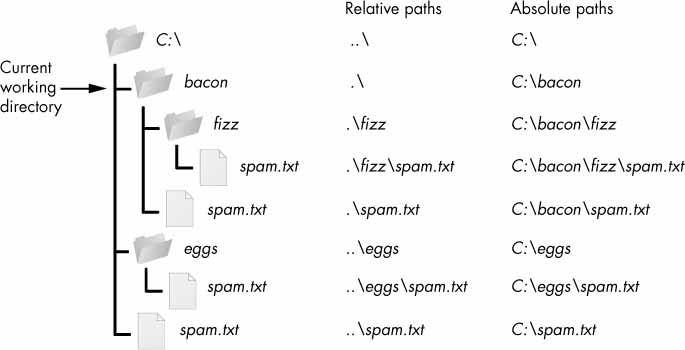
\includegraphics{./images/paths.jpeg}
\caption{Vir: \url{https://automatetheboringstuff.com/2e/chapter9/} (Al Sweigart, \href{https://creativecommons.org/licenses/by-nc-sa/3.0/}{CC BY-NC-SA 3.0})}
\end{figure}

Relativna pot do datoteke je pot glede na neko drugo mapo. Za zgornji primer:
glede na mapo \texttt{bacon} je relativna pot do datoteke \texttt{.\textbackslash{}fizz\textbackslash{}spam.txt}.

\begin{quote}
Pika pomeni trenutno mapo.
\end{quote}

Če bi bila trenutna mapa \texttt{eggs}, bi bila relativna pot do prejšnje datoteke
glede na \texttt{eggs} enaka \texttt{..\textbackslash{}bacon\textbackslash{}fizz\textbackslash{}spam.txt}.

\begin{quote}
Dve piki pomenita eno mapo višje v hierarhiji (parent folder) glede na trenutno mapo.
\end{quote}

Če bi želeli iti dve mapi višje bi uporabili \texttt{..\textbackslash{}..}, npr. iz mape
\texttt{fizz} v mapo \texttt{eggs} pridemo z \texttt{..\textbackslash{}..\textbackslash{}eggs}, itd.

Za podrobnejši razlago in več primerov glej gradivo: \url{https://automatetheboringstuff.com/2e/chapter9/}

\hypertarget{delo-z-ukaznim-pozivom}{%
\subsection{Delo z ukaznim pozivom}\label{delo-z-ukaznim-pozivom}}

Podobno kot v Raziskovalcu (File Explorer) se tudi v ukaznem pozivu (Terminal) v
nekem trenutku nahajamo v neki mapi (ang. Current working directory ali CWD).
Ta mapa je vedno napisana na začetku vrstice.
V ukaznem pozivu najprej napišemo ukaz nato parametre, ki jih želimo podati, ločene
s presledki. Ukaz izvedemo s tipko Enter.

V neko mapo se lahko premaknemo z ukazom \texttt{cd}, ki mu kot argument podamo pot
(relativno ali absolutno do mape, v katero se želimo premakniti.

Ukaz \texttt{dir} izpiše vse datoteke in mape, ki se nahajajo v trenutni mapi.

Glej tudi: \url{https://ucilnica.fmf.uni-lj.si/mod/page/view.php?id=2505}

\hypertarget{mape-in-datoteke-v-pythonu}{%
\subsection{Mape in datoteke v Pythonu}\label{mape-in-datoteke-v-pythonu}}

Za delo z datotečnim sistemom je na voljo knjižnica \texttt{os}.
Posamezne funkcije, njihove parametre in uporabo lahko poiščete v uradni
dokumentaciji ali drugod na spletu. Spodaj parametri funkcij niso napisani!

Nekaj najbolj uporabnih:

\begin{itemize}
\tightlist
\item
  \texttt{os.getcwd()} vrne trenutno mapo (CWD)
\item
  \texttt{os.chdir()} nastavi trenutno mapo na podano pot
\item
  \texttt{os.listdir()} vrne seznam poti do datotek in map, ki se nahajajo v mapi, do katere vodi pot
\item
  \texttt{os.mkdir()} ustvari novo mapo, ki se nahaja na podani poti
\item
  \texttt{os.rename()} preimenuje mapo, prvi parameter je pot mape, drugi pa nova pot (z novim imenom)
\item
  \texttt{os.remove()} izbriše datoteko, ki se nahaja na podani poti
\item
  \texttt{os.rmdir()} izbriše prazno mapo, ki se nahaja na podani poti
\end{itemize}

Za delo s potmi je na voljo knjižnica \texttt{os.path}, kjer so pogosto uporabljane funkcije:

\begin{itemize}
\tightlist
\item
  \texttt{os.path.exists()} vrne True, če podana pot obstaja
\item
  \texttt{os.path.join()} stakne dve poti v eno, pri čemer ustrezno poskrbi za prava ločila glede na OS
\item
  \texttt{os.path.abspath()} vrne absolutno pot, ki ustreza podani relativni poti (glede na trenutno mapo)
\item
  \texttt{os.path.relpath()} vrne relativno pot, ki ustreza podani absolutni poti (glede na trenutno mapo)
\item
  \texttt{os.path.isfile()} vrne True, če pot vodi do datoteke
\item
  \texttt{os.path.isdir()} vrne True, če pot vodi do mape
\end{itemize}

\hypertarget{pisanje}{%
\section{Pisanje}\label{pisanje}}

Datoteko odpremo v načinu za pisanje \texttt{mode="w"} in uporabimo funkcijo \texttt{write()},
ki zapiše niz v datoteko. Znak \texttt{\textbackslash{}n} pomeni novo vrstico. Če želimo zapisati znak \texttt{\textbackslash{}}
moramo v Pythonu napisati \texttt{\textbackslash{}\textbackslash{}}. Več o uporabi \texttt{\textbackslash{}} v Pythonu: \url{https://www.w3schools.com/python/gloss_python_escape_characters.asp}

\begin{Shaded}
\begin{Highlighting}[]
\NormalTok{potdodatoteke }\OperatorTok{=} \StringTok{"datoteka.txt"}
\ControlFlowTok{with} \BuiltInTok{open}\NormalTok{(potdodatoteke, mode}\OperatorTok{=}\StringTok{"w"}\NormalTok{, encoding}\OperatorTok{=}\StringTok{"utf{-}8"}\NormalTok{) }\ImportTok{as}\NormalTok{ dat:}
\NormalTok{    dat.write(}\StringTok{"To je "}\NormalTok{)}
\NormalTok{    dat.write(}\StringTok{"en stavek.}\CharTok{\textbackslash{}n}\StringTok{To je drugi."}\NormalTok{)}
\end{Highlighting}
\end{Shaded}

\begin{verbatim}
## datoteka.txt
## To je en stavek.
## To je drugi.
\end{verbatim}

Namesto \texttt{dat.write("niz")} se lahko uporablja tudi \texttt{print("niz",\ file=dat)}, kjer
odprto datoteko podamo kot parameter.

\hypertarget{branje}{%
\section{Branje}\label{branje}}

\hypertarget{read}{%
\subsection{read()}\label{read}}

Datoteko odpremo v načinu za branje \texttt{mode="r"} in uporabimo metodo \texttt{read()},
ki vrne celotno vsebino datoteke naenkrat v obliki niza.

\begin{Shaded}
\begin{Highlighting}[]
\ControlFlowTok{with} \BuiltInTok{open}\NormalTok{(}\StringTok{"datoteka.txt"}\NormalTok{, mode}\OperatorTok{=}\StringTok{"r"}\NormalTok{, encoding}\OperatorTok{=}\StringTok{"utf{-}8"}\NormalTok{) }\ImportTok{as}\NormalTok{ datoteka:}
\NormalTok{    vsebina }\OperatorTok{=}\NormalTok{ datoteka.read()}
\BuiltInTok{print}\NormalTok{(vsebina)}
\end{Highlighting}
\end{Shaded}

\begin{verbatim}
## To je en stavek.
## To je drugi.
\end{verbatim}

Uporaba argumenta \texttt{mode} je opisana na dnu strani.
Klicu \texttt{open} lahko podamo tudi neobvezni argument \texttt{encoding}, ki poda kodno
tabelo, v kateri je napisana datoteka. Privzeta vrednost tega argumenta je na
šolskih (in najverjetneje tudi vaših) Windows računalnikih \texttt{windows-1252}, kar je
nekoliko zastarel standard. Zato je dobra praksa uporaba parametra
\texttt{encoding="utf-8"}, s čimer uporabimo Unicode, ki se danes
uporablja skoraj povsod. Na macOS in Linux je vrednost \texttt{utf-8} že privzeta.

\hypertarget{readlines}{%
\subsection{readlines()}\label{readlines}}

Z metodo \texttt{readlines()} dobimo seznam, v katerem so posamezne
vrstice iz datoteke.

\begin{Shaded}
\begin{Highlighting}[]
\ControlFlowTok{with} \BuiltInTok{open}\NormalTok{(}\StringTok{"datoteka.txt"}\NormalTok{, mode}\OperatorTok{=}\StringTok{"r"}\NormalTok{, encoding}\OperatorTok{=}\StringTok{"utf{-}8"}\NormalTok{) }\ImportTok{as}\NormalTok{ datoteka:}
\NormalTok{    vrstice }\OperatorTok{=}\NormalTok{ datoteka.readlines()}
\BuiltInTok{print}\NormalTok{(vrstice)}
\end{Highlighting}
\end{Shaded}

\begin{verbatim}
## ['To je en stavek.\n', 'To je drugi.']
\end{verbatim}

\hypertarget{zanka}{%
\subsection{zanka}\label{zanka}}

Po vrsticah datoteke lahko gremo z zanko for.

\begin{Shaded}
\begin{Highlighting}[]
\NormalTok{vrstice }\OperatorTok{=}\NormalTok{ []}
\ControlFlowTok{with} \BuiltInTok{open}\NormalTok{(}\StringTok{"datoteka.txt"}\NormalTok{, mode}\OperatorTok{=}\StringTok{"r"}\NormalTok{, encoding}\OperatorTok{=}\StringTok{"utf{-}8"}\NormalTok{) }\ImportTok{as}\NormalTok{ datoteka:}
    \ControlFlowTok{for}\NormalTok{ line }\KeywordTok{in}\NormalTok{ datoteka:}
\NormalTok{        vrstice.append(line)}
\BuiltInTok{print}\NormalTok{(vrstice)}
\end{Highlighting}
\end{Shaded}

\begin{verbatim}
## ['To je en stavek.\n', 'To je drugi.']
\end{verbatim}

\hypertarget{mode}{%
\section{Mode}\label{mode}}

je neobvezni argument funkcije \texttt{open()}. Privzeta vrednost je \texttt{mode="rt"}. Zato
nam v zgornjih primerih ni bilo treba pisati \texttt{t} (je že privzet poleg druge
črke, ki jo podamo (\texttt{r} ali \texttt{w})). S posameznimi črkami povemo, kaj želimo z
datoteko početi.

\begin{longtable}[]{@{}
  >{\raggedright\arraybackslash}p{(\columnwidth - 4\tabcolsep) * \real{0.1111}}
  >{\raggedright\arraybackslash}p{(\columnwidth - 4\tabcolsep) * \real{0.4444}}
  >{\raggedright\arraybackslash}p{(\columnwidth - 4\tabcolsep) * \real{0.4444}}@{}}
\toprule()
\begin{minipage}[b]{\linewidth}\raggedright
oznaka
\end{minipage} & \begin{minipage}[b]{\linewidth}\raggedright
opis
\end{minipage} & \begin{minipage}[b]{\linewidth}\raggedright
opomba
\end{minipage} \\
\midrule()
\endhead
r & branje & če datoteka ne obstaja, sproži napako \\
w & pisanje & če datoteka ne obstaja, ustvari novo; če obstaja, izbriše prejšnjo vsebino datoteke \\
a & append & če datoteka ne obstaja, ustvari novo; če obstaja ne izbriše prejšnje vsebine \\
x & ustvari datoteko, pisanje & če datoteka že obstaja, sproži napako \\
+ & pisanje in branje & \\
t & za delo s tekstovnimi datotekami & npr. .txt, .csv, .tex, .html, .py \\
b & za delo s binarnimi datotekami & npr. slike \\
\bottomrule()
\end{longtable}

Nekaj lastnosti je zbranih v spodnji tabeli:

\begin{longtable}[]{@{}
  >{\raggedright\arraybackslash}p{(\columnwidth - 16\tabcolsep) * \real{0.4030}}
  >{\centering\arraybackslash}p{(\columnwidth - 16\tabcolsep) * \real{0.0746}}
  >{\centering\arraybackslash}p{(\columnwidth - 16\tabcolsep) * \real{0.0746}}
  >{\centering\arraybackslash}p{(\columnwidth - 16\tabcolsep) * \real{0.0746}}
  >{\centering\arraybackslash}p{(\columnwidth - 16\tabcolsep) * \real{0.0746}}
  >{\centering\arraybackslash}p{(\columnwidth - 16\tabcolsep) * \real{0.0746}}
  >{\centering\arraybackslash}p{(\columnwidth - 16\tabcolsep) * \real{0.0746}}
  >{\centering\arraybackslash}p{(\columnwidth - 16\tabcolsep) * \real{0.0746}}
  >{\centering\arraybackslash}p{(\columnwidth - 16\tabcolsep) * \real{0.0746}}@{}}
\toprule()
\begin{minipage}[b]{\linewidth}\raggedright
lastnost     \textbackslash{}     kombinacija črk
\end{minipage} & \begin{minipage}[b]{\linewidth}\centering
r
\end{minipage} & \begin{minipage}[b]{\linewidth}\centering
r+
\end{minipage} & \begin{minipage}[b]{\linewidth}\centering
x
\end{minipage} & \begin{minipage}[b]{\linewidth}\centering
x+
\end{minipage} & \begin{minipage}[b]{\linewidth}\centering
w
\end{minipage} & \begin{minipage}[b]{\linewidth}\centering
w+
\end{minipage} & \begin{minipage}[b]{\linewidth}\centering
a
\end{minipage} & \begin{minipage}[b]{\linewidth}\centering
a+
\end{minipage} \\
\midrule()
\endhead
branje & x & x & & x & & x & & x \\
pisanje & & x & x & x & x & x & x & x \\
datoteka mora obstajati & x & x & & & & & & \\
datoteka ne sme obstajati & & & x & x & & & & \\
zbriše prejšnjo vsebino datoteke & & & & & x & x & & \\
pisanje na konec datoteke & & & & & & & x & x \\
\bottomrule()
\end{longtable}

K zgornjim kombinacijam lahko dodamo še \texttt{t} ali \texttt{b}.

\end{document}
